\documentclass[xcolor=dvipsnames,compress,italian]{beamer}
\usetheme{Necst}

\begin{document}

\title[RAID, LVM, LUKS]{RAID, LVM, LUKS: Play with disks.}
		
\author[M. Polino]{Mario Polino}
\institute{
\vspace{1cm}
\begin{columns} 
    \begin{column}{0.30\columnwidth}
        \includegraphics[width=0.6\columnwidth]{img/PoliMI.eps}\hfill
    \end{column}
    \begin{column}{0.40\columnwidth}
        \centering \scriptsize{Corsi Avanzati Linux - 2014}
    \end{column}
    \begin{column}{0.30\columnwidth}
        \hfill
\includegraphics[width=\columnwidth]{img/poul.pdf}
    \end{column}
\end{columns}
}

\date{}

\frame[plain]{\vspace{1.1cm}\titlepage} 

\section[RAID]{ RAID }
\subsection{Intro}
\frame{\frametitle{RAID What?} 
	\begin{center}
		\includegraphics<1>[height=0.8\textheight]{./img/raid/raidcolor.jpg}
		\includegraphics<2>[height=0.8\textheight]{./img/raid/raidno.jpg}
	\end{center}	
}

\frame{\frametitle{RAID} 
	\begin{block}{Redundant Array of Inexpensive(Independent) Disks}
		\begin{itemize}
			\item[ITA] un sistema informatico che usa un gruppo di dischi rigidi per condividere o replicare le informazioni
			\item[ENG] schemes that can divide and replicate data among \textbf{multiple physical drives}
		\end{itemize}
	\end{block}

}

\subsection{Theory}

\frame{\frametitle{RAID 0: Striping}

\begin{columns} 
	\begin{column}{0.5\columnwidth}
		\begin{block}{Pros}
			\begin{itemize}
			 \item Alte prestazioni in scrittura e lettura.
			\end{itemize}
		\end{block}
		\begin{alertblock}{Cons}
			\begin{itemize}
			 \item Impossibile montare dischi hot-spare. 
			 \item Affidabilità minore di un disco singolo. 
			 \item Non è fault tolerant.
			\end{itemize}
		\end{alertblock}
	\end{column}
	\begin{column}{0.5\columnwidth}
		\begin{center}
			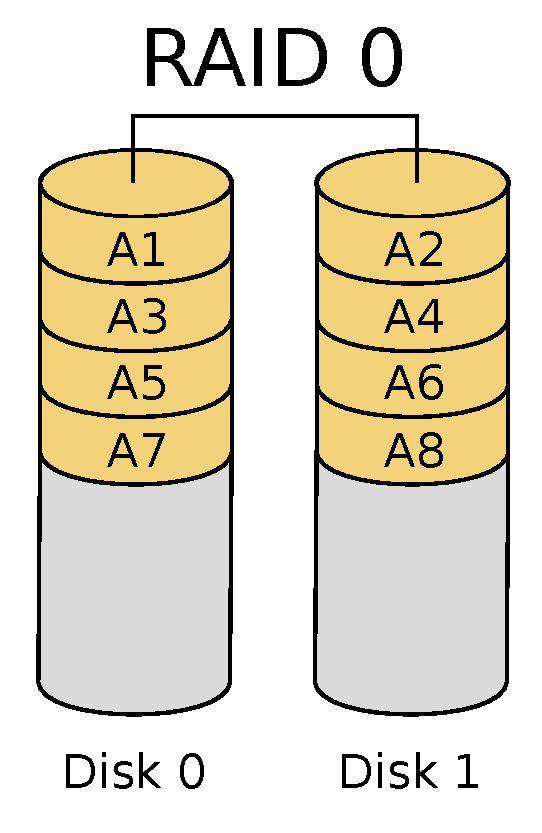
\includegraphics[height=0.8\textheight]{./img/raid/RAID_0.pdf}
		\end{center}
	\end{column}
	
\end{columns} 

}


\frame{\frametitle{RAID 1: Mirroring}

\begin{columns} 

	\begin{column}{0.5\columnwidth}
		\begin{center}
			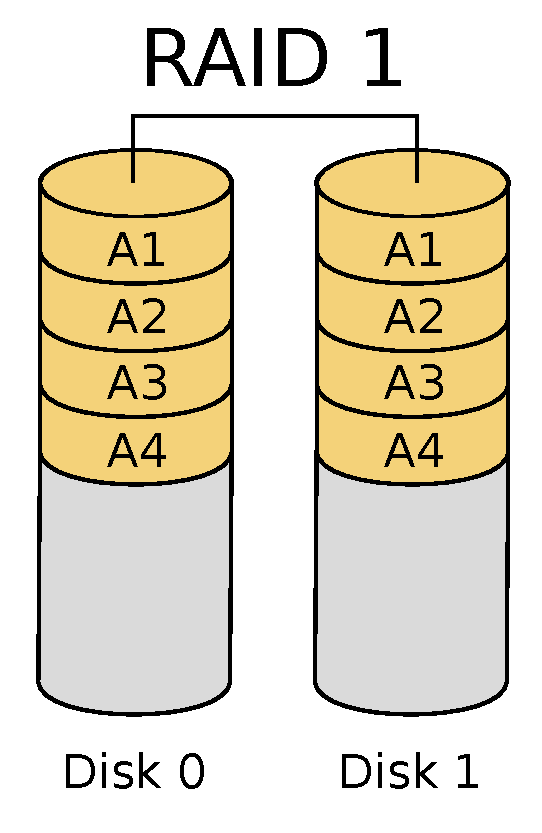
\includegraphics[height=0.8\textheight]{./img/raid/RAID_1.pdf}
		\end{center}
	\end{column}
	\begin{column}{0.5\columnwidth}
		\begin{block}{Pros}
			\begin{itemize}
			 \item Affidabilità proporzionale al numero di dischi.
			 \item Fault tolerance.
			 \item Velocità di lettura dipende dal disco più veloce
			\end{itemize}
		\end{block}
		\begin{alertblock}{Cons}
			\begin{itemize}
			 \item Alto costo. 
			 \item Velocità di scrittura dipende dal disco più lento.
			\end{itemize}
		\end{alertblock}


	\end{column}
	
\end{columns} 

}

\frame{\frametitle{RAID 2,3: Never Implemented}
	\begin{center}
		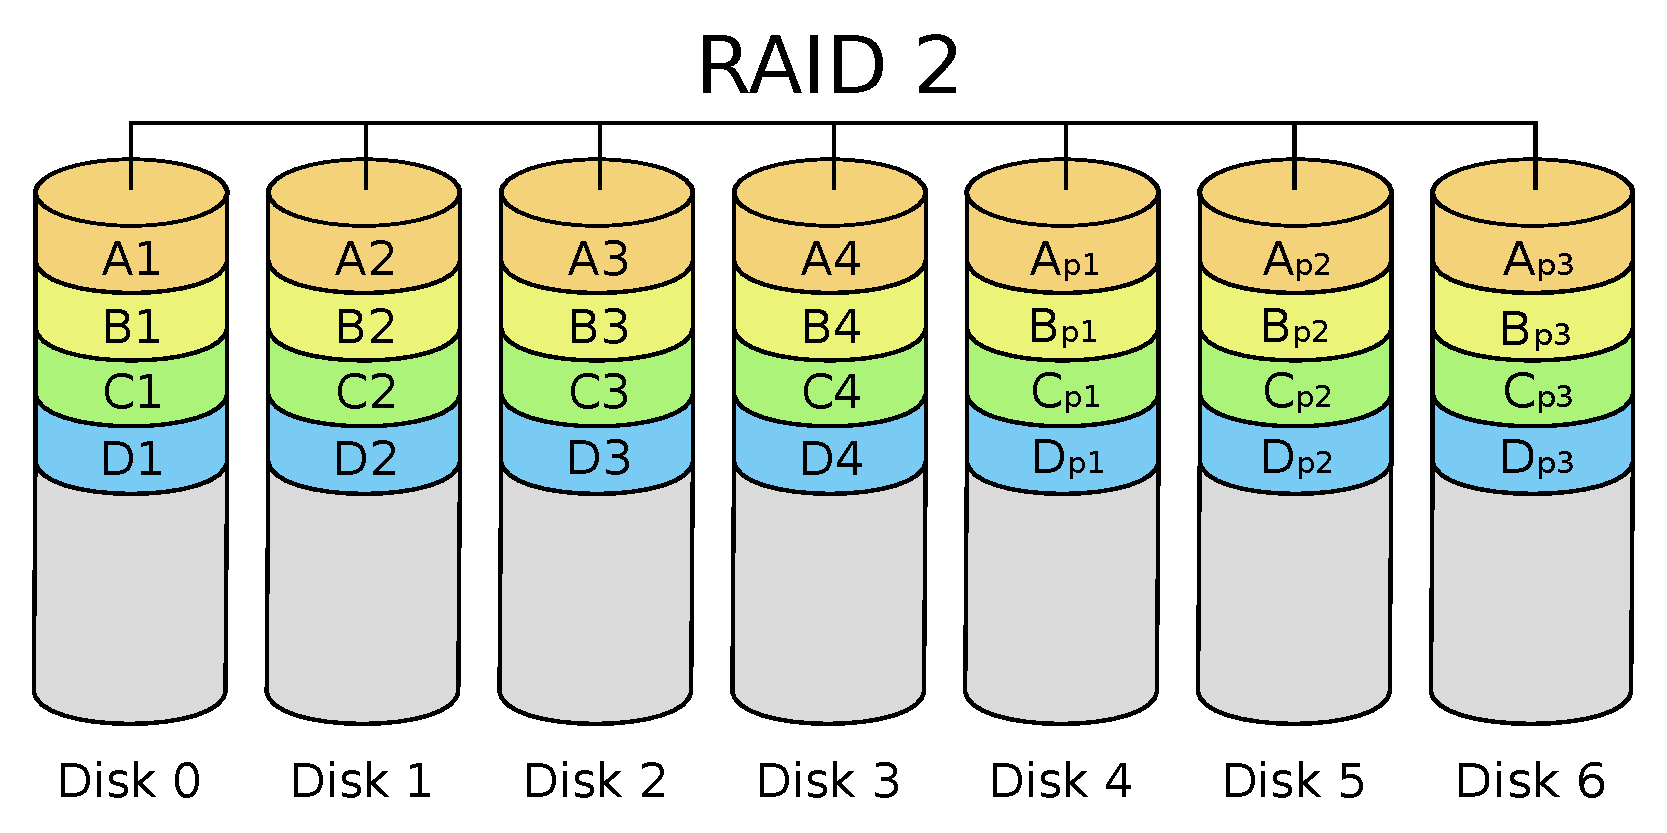
\includegraphics[height=0.4\textheight]{./img/raid/RAID_2.pdf}
	\end{center}
	\begin{center}
		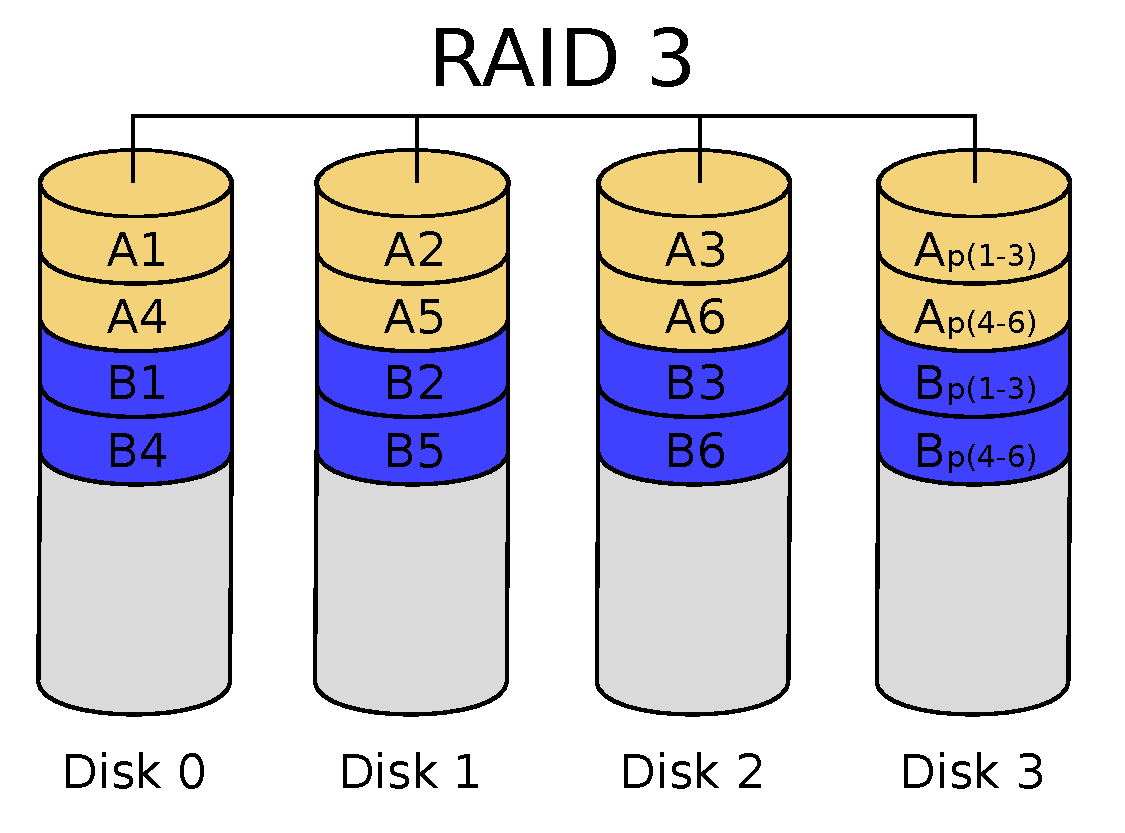
\includegraphics[height=0.4\textheight]{./img/raid/RAID_3.pdf}
	\end{center}

}

\frame{\frametitle{RAID 4: Block Level Striping with Dedicated Parity Disk}
\begin{columns} 
	\begin{column}{0.5\columnwidth}
		\begin{center}
			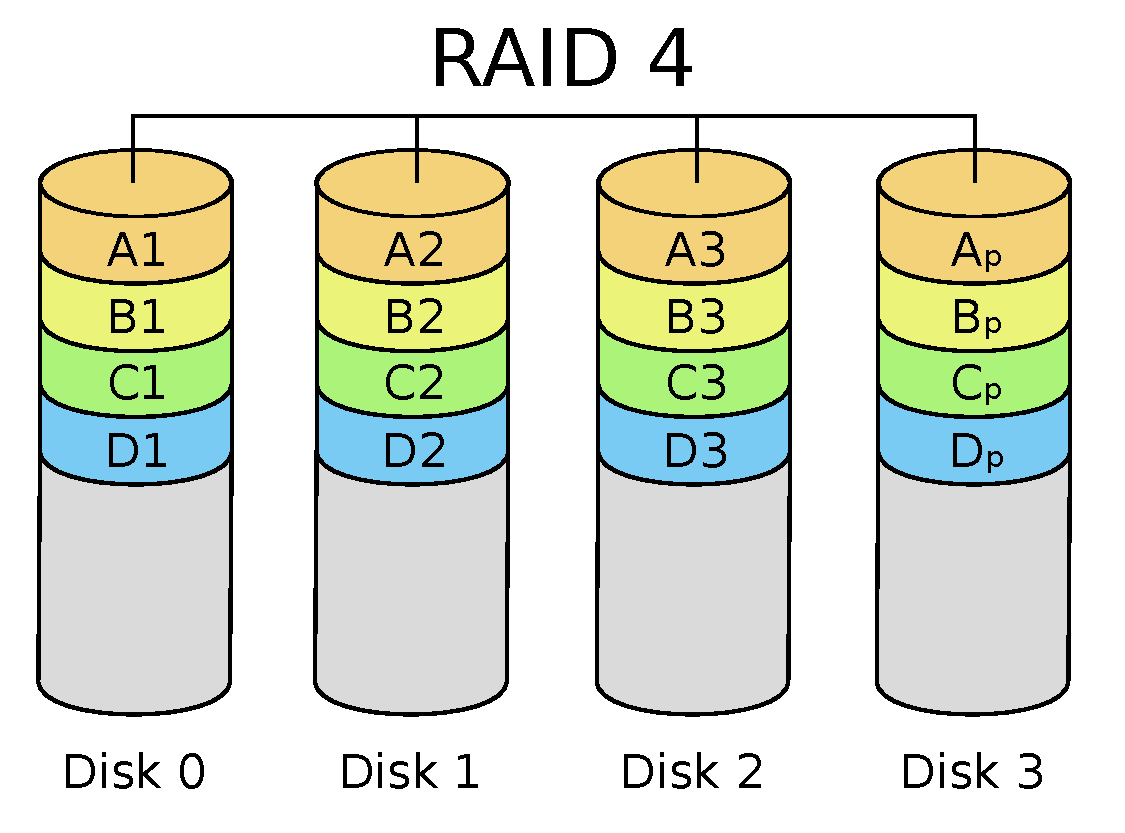
\includegraphics[width=0.9\textwidth]{./img/raid/RAID_4.pdf}
		\end{center}
	\end{column}
	\begin{column}{0.5\columnwidth}
		\begin{block}{Pros}
			\begin{itemize}
			 \item Read veloci grazie al parallelismo della struttura.
			 \item Fault tolerance.
			 \item Possibilità di inserire dischi hot-spare.
			\end{itemize}
		\end{block}
	\end{column}
\end{columns}

	\begin{alertblock}{Cons}
		\begin{itemize}
		 \item Il disco utilizzato per la parità è il collo di bottiglia. 
		 \item Scrittura lenta a causa del calcolo della parità
		\end{itemize}
	\end{alertblock}

}

\frame{\frametitle{RAID 5: Block Level Striping with Distributed Parity}
\begin{columns} 
	\begin{column}{0.5\columnwidth}
		\begin{block}{Pros}
			\begin{itemize}
			 \item Read veloci grazie al parallelismo della struttura.
			 \item Fault tolerance.
			 \item Possibilità di inserire dischi hot-spare.
			\end{itemize}
		\end{block}
	\end{column}
	\begin{column}{0.5\columnwidth}
		\begin{center}
			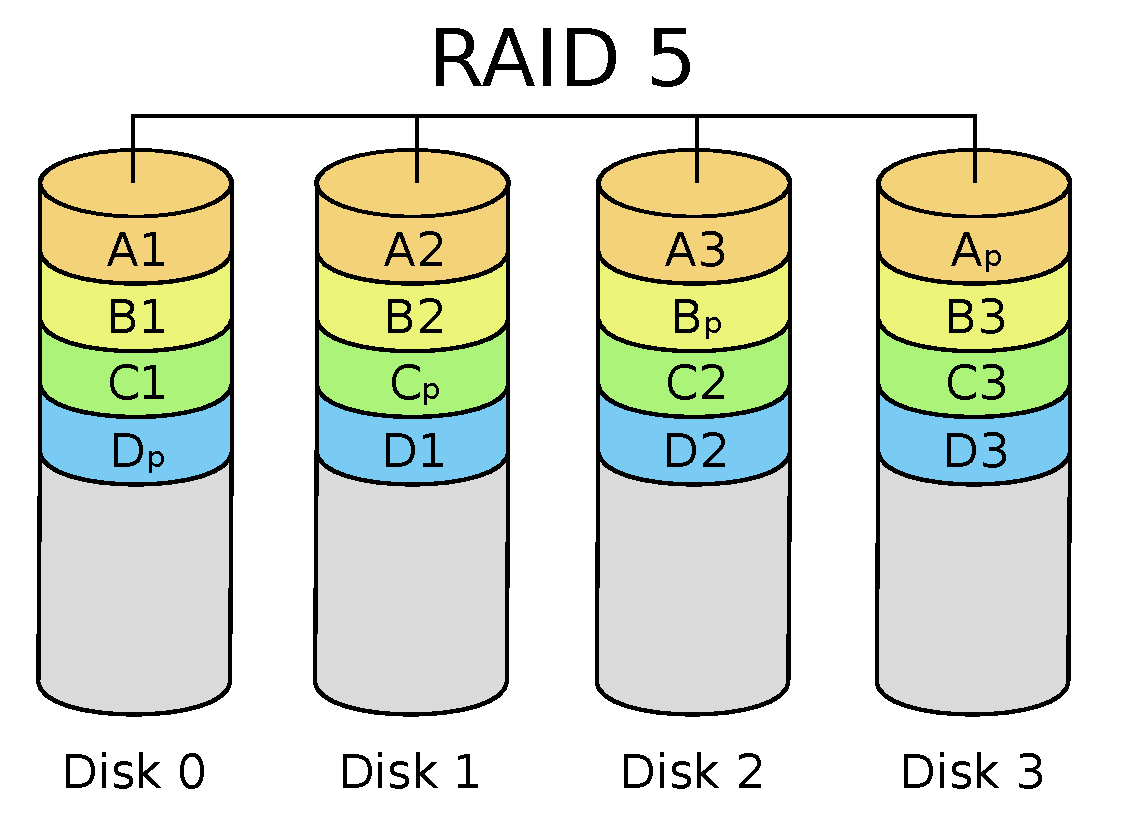
\includegraphics[width=0.9\textwidth]{./img/raid/RAID_5.pdf}
		\end{center}
	\end{column}

\end{columns}

	\begin{alertblock}{Cons}
		\begin{itemize}
		 \item Scrittura lenta a causa del calcolo della parità
		\end{itemize}
	\end{alertblock}

}

\frame{\frametitle{RAID 6: Block Level Striping with Double Distributed Parity}
\begin{columns} 
	\begin{column}{0.5\columnwidth}
		\begin{block}{Pros}
			\begin{itemize}
			 \item Read veloci grazie al parallelismo della struttura.
			 \item Fault tolerance.
			 \item Possibilità di inserire dischi hot-spare.
			\end{itemize}
		\end{block}
	\end{column}
	\begin{column}{0.5\columnwidth}
		\begin{center}
			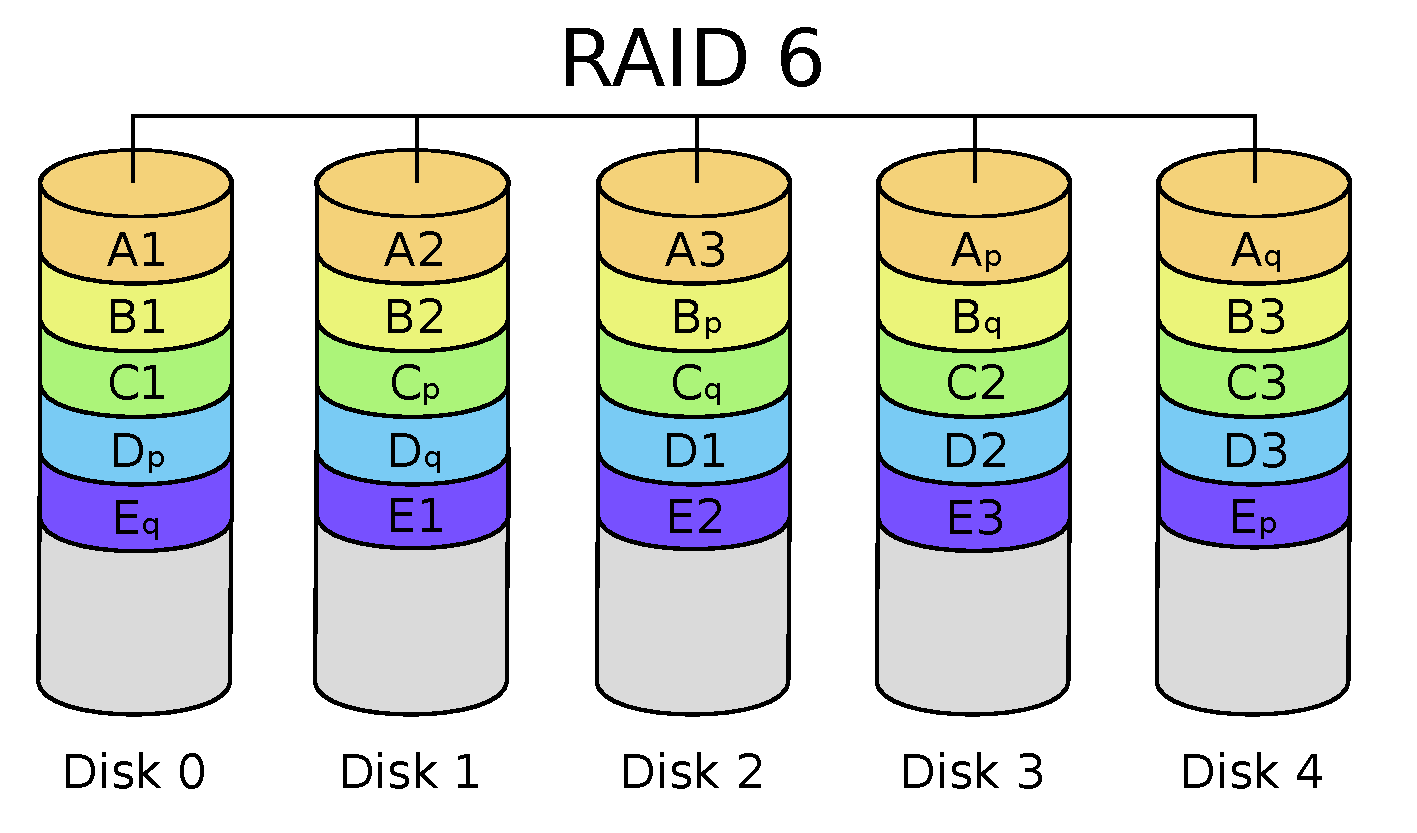
\includegraphics[width=0.9\textwidth]{./img/raid/RAID_6.pdf}
		\end{center}
	\end{column}

\end{columns}

	\begin{alertblock}{Cons}
		\begin{itemize}
		 \item Scrittura \emph{`molto'} lenta a causa del calcolo della parità
		\end{itemize}
	\end{alertblock}

}

\frame{\frametitle{RAID 0+1 vs 1+0}
\begin{columns} 
	\begin{column}{0.5\columnwidth}
		\begin{center}
			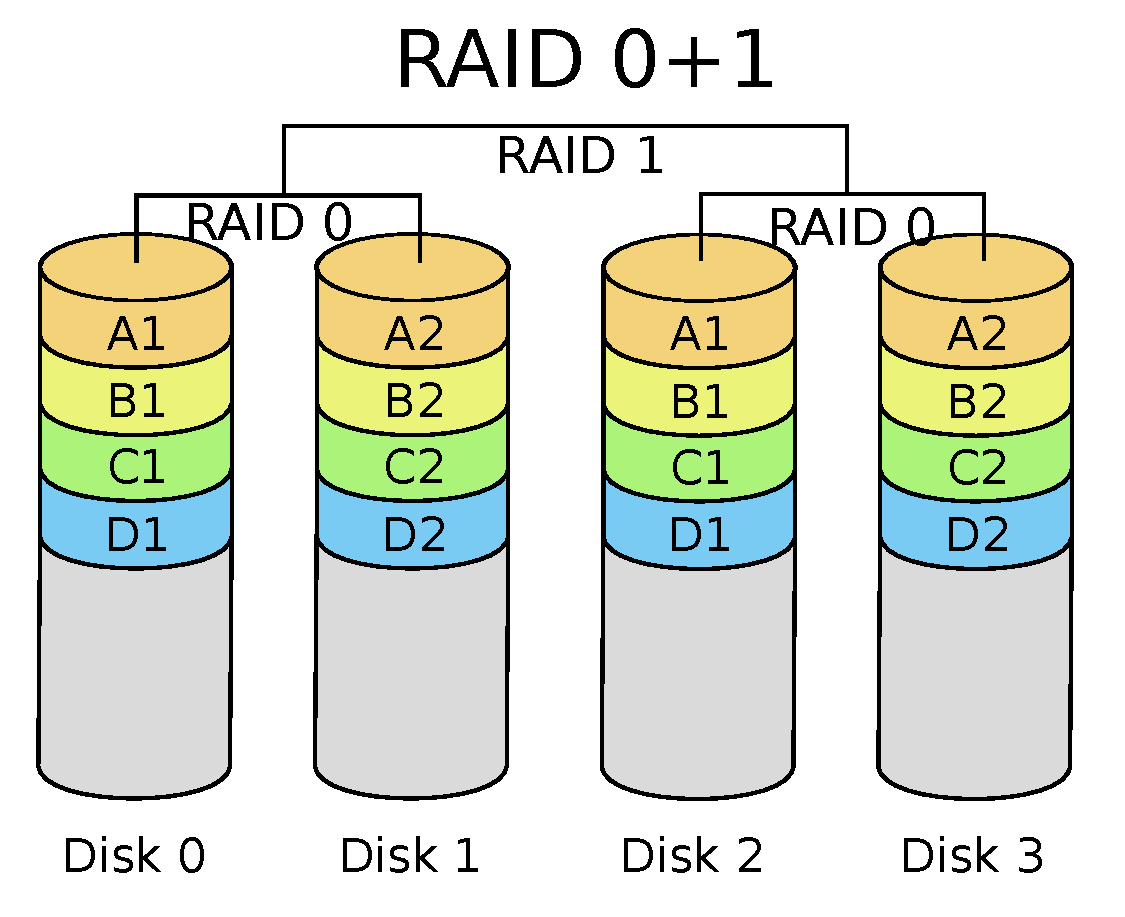
\includegraphics[width=0.9\textwidth]{./img/raid/RAID_01.pdf}
		\end{center}
	\end{column}
	\begin{column}{0.5\columnwidth}
		\begin{center}
			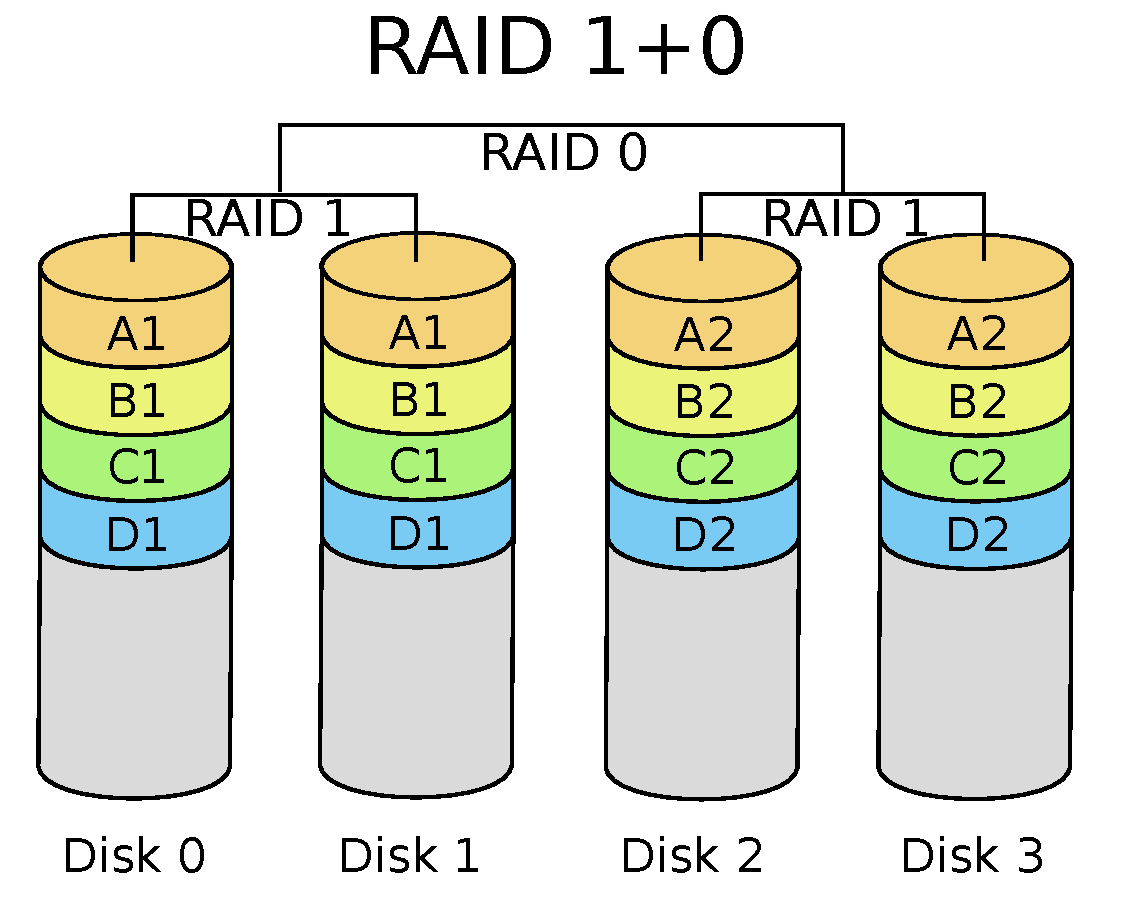
\includegraphics[width=0.9\textwidth]{./img/raid/RAID_10.pdf}
		\end{center}
	\end{column}

\end{columns}

	\begin{alertblock}{}
		\begin{itemize}
		 \item 1+0 è una scelta migliore.
		\end{itemize}
	\end{alertblock}

}
\subsection{mdadm}

\frame{\frametitle{mdadm - manage MD devices aka Linux Software RAID}
\begin{block}
\Large {mdadm [mode] <raiddevice> [options] <component-devices>}
\end{block}
}

\frame{\frametitle{mdadm - Supporto}
	\begin{itemize}
	 \item RAID\textbf{0}
	 \item RAID\textbf{1}
	 \item RAID\textbf{4}
	 \item RAID\textbf{5}
	 \item RAID\textbf{6}
	 \item RAID\textbf{10} (1 + 0)
	 \item LINEAR (Come RAID0 con dischi di dimensione diversa)
	\end{itemize}
}

\frame{\frametitle{mdadm - mode}
	\begin{itemize}
		\item[-A] Assemble: Assembla i componenti di un array già creato in un block device attivo.
		\item[-C] Create: Crea un nuovo array di dischi e lo attiva.
		\item[-F] Follow/Monitor: Controlla lo stato dei dischi.
		\item[-G] Grow: Cambia il numero di dischi il layout, etc.
	\end{itemize}
}

\frame{\frametitle{mdadm - Create}

 \begin{block}{}
 \Large {mdadm -Cv /dev/md0 --level=5 --raid-devices=3 /dev/sdb1 /dev/sdc1 /dev/sdd1 --spare-devices=1 /dev/sde1}
 \end{block}
 }

\frame{\frametitle{mdadm - Add/Remove per un Disco}

\begin{block}{Add}
 \Large {mdadm --add /dev/md0 /dev/sdb1}
 \end{block}

\begin{block}{Remove}
 \Large {mdadm /dev/md0 --fail /dev/sda1 --remove /dev/sda1}
 \end{block}
 }
\frame{\frametitle{mdadm - Monitorare un Array}

\begin{block}{}
 \Large {mdadm --detail /dev/md0}
\end{block}

\begin{block}{}
 \Large {cat /proc/mdstat}
\end{block}

\begin{alertblock}{}
Personalities : [raid1]\\
md0 : active raid1 sdb1[1] sda1[0]\\
104320 blocks [2/2] [UU]\\

md1 : active raid1 sdb3[1] sda3[0]\\
19542976 blocks [2/2] [UU]\\

md2 : active raid1 sdb4[1] sda4[0]\\
223504192 blocks [2/2] [UU]\\
\end{alertblock}
 }

\frame{\frametitle{mdadm - Stop/Delete per un Array}

\begin{block}{Stop}
 \Large {mdadm --stop /dev/md0}
 \end{block}

\begin{block}{Delete}
 \Large {mdadm --remove /dev/md0}
 \end{block}
 }

\frame{\frametitle{mdadm - /etc/mdadm.conf}
	\begin{block}{}
	 mdadm --examine --scan > /etc/mdadm.conf

	\end{block}

}

% \frame[plain]{\frametitle{}
% 	\huge{Demo}
% }	


\section{LVM}
\subsection{Theory}

\frame{\frametitle{Cosa è LVM?}
	\begin{columns}
		\begin{column}{0.5\columnwidth}
			\begin{block}{\textbf{L}ogical \textbf{V}olume \textbf{M}anager}
			Crea un livello di astrazione che permette di creare dischi logici che vengono poi archiviati in dischi fisici.
			\end{block}
		\end{column}
		\begin{column}{0.5\columnwidth}

			\begin{center}
				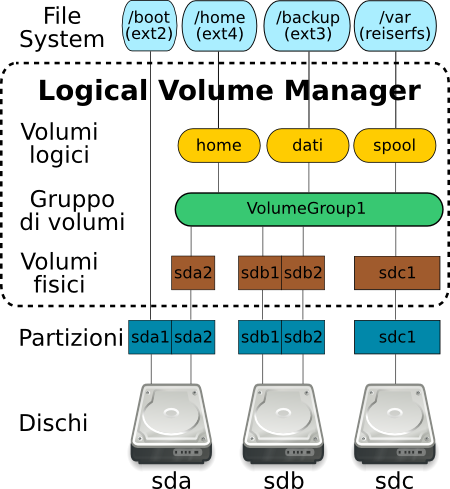
\includegraphics[width=\textwidth]{./img/LVM/lvm1.png}
			\end{center}
		\end{column}
	\end{columns}
}

% \frame{\frametitle{Cosa è LVM?}
% 	\begin{center}
% 		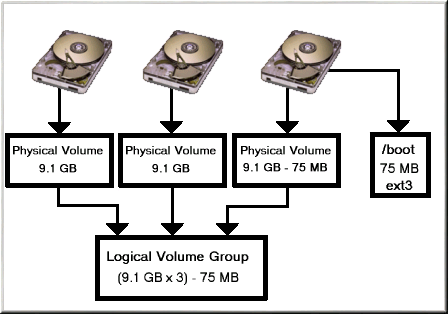
\includegraphics[width=0.5\textwidth]{./img/LVM/lvg.png}
% 	\end{center}

% }
\frame{\frametitle{I Vantaggi di LVM}

	\begin{itemize}
    \item \textbf{Capacità flessibile}: Un Filesystem può essere esteso su più dischi fisici.
    \item \textbf{Storage ridimensionabile}: Si può fare il redimensionamento dei volumi logici senza intaccare le partizioni.
    \item \textbf{Online data relocation}: Puoi riposizionare i dati mentra il sistama è attivo. Per esempio puoi decidere di svuotare completamente un disco prima di rimuoverlo.

    \item \textbf{Nomi significativi}: I volumi possono essere raggruppati e nominati a piacimento dell'utente.

    \item \textbf{Disk striping}: Simile al RAID0

    \item \textbf{Mirroring volumes}: Simile al RAID1

    \item \textbf{Volume Snapshot}: Si possono creare snapshot dei volumi (e quindi fare modifiche che non modificano i dati reali)

    \end{itemize}
	
}
\subsection{Commands}

\frame{\frametitle{lvm - Gestire i volumi fisici}

\begin{block}{pvcreate /dev/sda2}
  inizializza la partizione \emph{/dev/sda2} per l'uso di LVM (Si può usare anche su interi dischi)
 \end{block}

\begin{alertblock}{pvscan}
	pvscan scans all supported LVM block devices in the system for physical volumes.
 \end{alertblock}

\begin{alertblock}{pvdisplay}
  Mostra le informazioni su un volume fisico
 \end{alertblock}



 }


\frame{\frametitle{lvm - Creare gruppi di volumi}

\begin{block}{vgcreate VolGroup00 /dev/sda2}
  Crea un nuovo gruppo di volumi di nome \emph{VolGroup00} che contiene il disco \emph{/dev/sda2}
 \end{block}

\begin{block}{vgextend VolGroup00 /dev/sdb1}
	Aggiunge la partizione \emph{/dev/sdb1} al gruppo \emph{VolGroup00}
 \end{block}

\begin{alertblock}{vgscan}
	Legge tutti i dischi alla ricerca di volumi fisici che contengono metadati di LVM.
 \end{alertblock}

 \begin{alertblock}{vgdisplay}
 	Mostra informazioni sui Volume Group
 \end{alertblock}
 }

\frame{\frametitle{lvm - Creare i volumi logici lineari}

\begin{block}{lvcreate -L 10G VolGroup00 -n lvolhome}
  Crea un volume logico di 10GB nome \emph{lvolhome}\\
  Il volume è accessibile da \emph{/dev/mapper/VolGroup00-lvolhome} o \emph{/dev/VolGroup00/lvolhome}\\
  Si può usare l'opzione \emph{-C y} per assicurarsi che il volume sia contiguo. 
 \end{block}

\begin{block}{lvcreate -l +100\%FREE VolGroup00 -n lvolmedia}
  Crea un volume logico che occupa tutto il restante spazio disponibile \\
 \end{block}

 \begin{alertblock}{lvdisplay}
 	Mostra informazioni sui Volumi logici
 \end{alertblock}
 }

\frame{\frametitle{lvm - Creare i volumi logici stripped}

	\begin{center}
		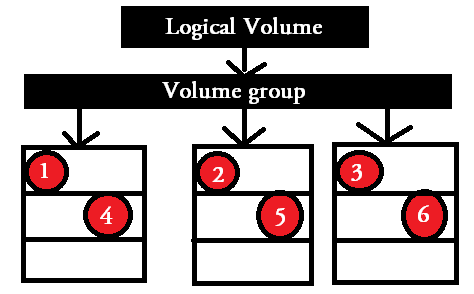
\includegraphics[width=0.5\textwidth]{./img/LVM/stripped.png}
	\end{center}

	\begin{block}{lvcreate -L 10G \textbf{-i2 -I64} -n example VolGroup00}
	 Crea un volume logico stile RAID 0 con blocchi di dimensione di 64 kb, dimensione 10G, usando due volumi fisici. 
	 \end{block}

	\begin{alertblock}{}
		Hai bisogno di \textbf{almeno 2} volumi fisici
	 \end{alertblock}
 }

 \frame{\frametitle{lvm - Creare i volumi logici mirrored}
	\begin{columns}
	 	\begin{column}{0.5\columnwidth}
			\begin{center}
				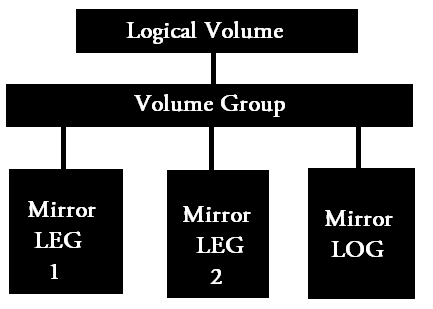
\includegraphics[width=\textwidth]{./img/LVM/mirrored.png}
			\end{center}
		\end{column}
	 	\begin{column}{0.5\columnwidth}
			\begin{alertblock}{}
				Hai bisogno di \textbf{almeno 3} volumi fisici, il terzo è usato per log relativi al mirroring
			 \end{alertblock}
 			\begin{block}{lvconvert -m1 /dev/vg00/lv0}
 				Il mirroring può essere aggiunto o eliminato (-m0) anche da un volume già esistente 
			 \end{block}

		\end{column}


	\end{columns}
	\begin{block}{lvcreate -L 10G \textbf{-m1} -n mirrorexample VolGroup00}
	 Crea un volume logico con un mirror (stile RAID 1) di dimensione 10G. 
	 \end{block}
 }


\frame{\frametitle{lvm - Snapshot}

\begin{block}{COW (copy-no-write)}
	Lo snapshot iniziale conterrà hard-link agli inode dei dati attuali. Fino a che i dati restano invariati, lo snapshot conterrà solo i link agli inode e non i dati stessi. Quando verrà modificato un file o una cartella ai quali lo snapshot punta, LVM automaticamente clonerà i dati, la vecchia copia referenziata dallo snapshot, e la nuova copia referenziata dall'attuale sistema.
 \end{block}

\begin{block}{lvcreate --size 100M --snapshot --name snap01 /dev/mapper/vg0-pv}
	Crea un nuovo volume logico basato su \emph{/dev/mapper/vg0-pv} con massi 100MB di modifiche apportabili.
 \end{block}


 }

\section{LUKS}

\subsection{Theory}

\frame{\frametitle{Cosa è LUKS?}

			\begin{center}
				
\includegraphics[width=0.7\textwidth]{./img/LUKS/luks-logo.png}
			\end{center}


			\begin{block}{\textbf{L}inux \textbf{U}nified \textbf{K}ey \textbf{S}etup}
				è lo standard per hard disk cifrati su linux. 
			\end{block}

}
\frame{\frametitle{I Vantaggi di LUKS}

			\begin{block}{}
				\begin{itemize}
					\item Compatibilità via standardizzazione.
    				\item Sicuro contro attacchi low entropy.
    				\item Supporto per multi key.
    				\item Effective passphrase revocation.
    				\item Free 
				\end{itemize}
			\end{block}
}


\frame{\frametitle{Wipe the Disk}


			\begin{block}{cat /dev/zero > /dev/sdx}
				Scrive zero sul disco \emph{sdx}.\\
				Se il disco è stato usato in precedenza, è una buona idea fare un wipe prima di creare un LUKS
				container per rimuovere ogni traccia del vecchio filesystem e dei vecchi dati.
			\end{block}

			\begin{block}{}
				dd if=/dev/urandom of=/dev/sdx
			\end{block}

			\begin{alertblock}{Flash memory/SSD}
				Le memorie SSD e/o flash adottano un livello di astrazione per cui i dati non sono scritti esattamente nel settore indicato. Alcuni fanno addirittura la compressione dei dati, quindi scrivere solo zeri risulta in avere sovrascritto poco spazio. \url{https://www.usenix.org/legacy/events/fast11/tech/full_papers/Wei.pdf}
			\end{alertblock}

}

\frame{\frametitle{The Command}

	\begin{block}{}
		cryptsetup <OPTIONS> <action> <action-specific> <device> <dmname>
	\end{block}

	\begin{block}{Mode}
		\begin{itemize}
			\item \textbf{LUKS}: Default 
			\item plain: Per usare dm-crypt in plain mode  
			\item loopaes: legacy mode 
			\item tcrypt: Modo compatibile con Truecrypt 

		\end{itemize}
	\end{block}
}

\frame{\frametitle{Format/Open}

	\begin{block}{cryptsetup -v --cipher aes-xts-plain64 --key-size 512 --hash sha1 --iter-time 1000 \textbf{luksFormat} <device> }
		\emph{--chiper} per impostare il cifrario da usare (aes-xts-plain64)\\
		\emph{--key-size} dimensione della chiave (256)\\
		\emph{--hash} funzione di hash per PBKDF2 (sha1)\\
		\emph{--iter-time} numero di millisecondi spesi dentro PBKDF2 (1000)\\
	\end{block}

	\begin{block}{cryptsetup \textbf{open --type luks} /dev/sdx chipDevice}
			Apre la partizione cifrata \emph{sdx} creando un device a blocchi \emph{/dev/mapper/chipDevice} che si può utilizzare come un normale disco.
	\end{block}
}
\frame{\frametitle{Keyfiles}

	\begin{block}{dd if=/dev/urandom of=mykeyfile bs=512 count=4}
		Genera un file \emph{mykeyfile} e lo riempie di dati random
	\end{block}

	\begin{block}{cryptsetup -c <desired cipher> -s <key size> luksFormat /dev/<volume to encrypt> \textbf{/path/to/mykeyfile}}
		Crea un disco cifrato e usa \emph{mykeyfile} come chiave di cifratura.
	\end{block}

	\begin{block}{cryptsetup \textbf{open --type luks} --key-file \textbf{/path/to/mykeyfile}  /dev/sdx chipDevice}
			Apre la partizione cifrata \emph{sdx} usanto \emph{mykeyfile} come file.
	\end{block}
	\begin{block}{}
	\footnotesize Si può utilizzare come chiave sia un file che un device a blocchi (una partizione, magari su un dispositivo rimovibile). Si può utilizzare l'opzione \emph{--keyfile-offset} per indicare l'offset di inizio della chiave sul file/dispositivo e \emph{--keyfile-size} per indicare la quantità di dati da considerare per la chiave.
	\end{block}
}

\frame{\frametitle{Key management /1}

	\begin{alertblock}{}
		Si possono usare fino a \textbf{8} chiavi differenti. I key slot vanno da 0 a 7
	\end{alertblock}

	\begin{block}{cryptsetup luksDump /dev/<device>}
		Informazioni sul device cifrato e sulle chiavi utilizzate
	\end{block}

	\begin{block}{cryptsetup luksAddKey /dev/<device> [/path/to/<additionalkeyfile>] [-d /path/to/<keyfile>]}
		Aggiunge una nuova chiave nel primo slot libero. Per l'aggiunta di una nuova chiave bisogna essere in possesso di almeno una delle vecchie.\\
		\emph{-d} è usata per indicare il percorso del keyfile da utilizzare come chiave.\\
		\emph{-S} specifica lo slot nel quale si vuole aggiungere la chiave.
	\end{block}
}

\frame{\frametitle{Key management /2}

	\begin{block}{cryptsetup luksChangeKey /dev/<device> -S 6 }
		Cambia la chiave dello slot 6. Bisogna essere a conoscenza della chiave che si sta cambiando.
	\end{block}


	\begin{alertblock}{}
		Con entrambe le opzioni seguenti è possibile rimuovere anche l'ultima chiave rimasta e quindi rendere i dati persi per sempre.
	\end{alertblock}

	\begin{block}{cryptsetup luksRemoveKey /dev/<device>}
		Rimuove la chiave inserita.
	\end{block}

	\begin{block}{cryptsetup luksKillSlot /dev/<device> 6}
		Rimuove la chiave nello slot 6 con una qualsiasi altra chiave.
	\end{block}
}

\frame{\frametitle{Backup LUKS Header}

	\begin{alertblock}{}
		L'header della partizione cifrata è di vitale importanza per poter accedere hai dati contenuti, quindi un danno accidentale a questa sezione può rendere inaccessibili tutti i dati.
	\end{alertblock}

	\begin{block}{cryptsetup luksHeaderBackup /dev/sdx --header-backup-file /path/to/header.img}
		Salva in \emph{header.img} una copia di backup del header della partizione \emph{sdx}
	\end{block}
}
\frame{\frametitle{Restore LUKS Header}

	\begin{block}{cryptsetup -v --header /path/to/header.img open /dev/sdx testHead}
		Apre il device \emph{sdx} utilizzando l'header \emph{header.img}. Non sovrascrive l'header originale del device. \'E utile per controllare che l'header sia corretto prima di fare il Restore.
	\end{block}

	\begin{block}{cryptsetup luksHeaderRestore /dev/sdx --header-backup-file ./path/to/header.img}
		Sovrascrive l'header del dispositivo \emph{sdx} con il backup contenuto in \emph{header.img}
	\end{block}


}


\section*{}
\frame[plain]{\frametitle{}
	\huge{Grazie per l'attenzione.}
}	
\end{document}